\documentclass[11pt,a4paper]{article}

\usepackage[utf8]{inputenc}
\usepackage[T1]{fontenc}
\usepackage[margin=3cm]{geometry}
\usepackage{amsmath,amssymb,amsthm}
\usepackage{graphicx}
\usepackage{booktabs}
\usepackage{listings}
\usepackage{url}
\usepackage[hidelinks]{hyperref}
\hypersetup{
  pdftitle={Building New IFS Attractors: a Working Vocabulary of Affine Maps},
  pdfauthor={Cédric Bonhomme},
  pdfsubject={Construction techniques for the attractors of affine iterated function systems},
  pdfkeywords={iterated function systems, fractals, chaos game, attractor,
    self-similarity, phyllotaxis, golden angle, OCaml,
    doi:10.5281/zenodo.21804778}
}

\graphicspath{{figures/}}

\newtheorem{theorem}{Theorem}
\newtheorem{proposition}[theorem]{Proposition}
\newtheorem{lemma}[theorem]{Lemma}
\theoremstyle{remark}
\newtheorem{remark}[theorem]{Remark}

\lstset{basicstyle=\ttfamily\small, columns=fullflexible, keepspaces=true}

\newcommand{\R}{\mathbb{R}}
\newcommand{\Hs}{\mathcal{H}}

\title{Building New IFS Attractors:\\ a Working Vocabulary of Affine Maps}
\author{Cédric Bonhomme\\ \small\texttt{cedric@cedricbonhomme.org}}
\date{July 2026\\[0.6em]
  \small doi:\,\href{https://doi.org/10.5281/zenodo.21804778}%
  {10.5281/zenodo.21804778}}

\begin{document}

\maketitle

\begin{abstract}
The attractor of an affine iterated function system (IFS) is determined by a
handful of real coefficients, yet finding coefficients that produce a
\emph{desired} shape remains something of a dark art. We propose a design
grammar for the inverse problem: five named families of affine maps
(rank-deficient \emph{stem maps}, dominant rotation-contractions for spirals,
radial replication for umbrella-shaped inflorescences, golden-angle rotations
for phyllotaxis, and non-contracting \emph{symmetry maps}) that compose into
new attractors, together with the design loop that turns a family into
shipped coefficients. Six original attractors, all distributed in an OCaml
library, serve as witnesses. Symmetry maps leave the classical Hutchinson
framework and are admissible only under the average contractivity condition
of Barnsley, Demko and Elton; we show that this freedom is bounded by a
rigidity result, since an attractor whose system contains a scale-one
rotation is provably invariant under that rotation. That obstruction explains
why a symmetric idealization is the best an IFS can offer for a designed
symbol such as the Icelandic vegvísir, and motivates a closing discussion of
why grown, organic forms admit compact IFS descriptions while designed ones
resist them.
\end{abstract}

\section{Introduction}

Iterated function systems are the most economical fractal encoding we know
of: four affine maps, twenty-four real numbers, suffice to describe
Barnsley's fern in recognizable botanical detail
\cite{barnsleydemko1985,barnsley1988}. The theory is classical
\cite{hutchinson1981,falconer1990} and the classical examples are
well documented \cite{vrscay,sester2017}. What is documented much less often
is the \emph{inverse} craft: given a shape in mind, how does one sit down and
write the coefficients? Barnsley's collage theorem \cite{barnsley1988} gives
the guiding principle (cover the target with small affine copies of itself)
but stops short of a design vocabulary.

This note records such a vocabulary, distilled from extending a small OCaml
program \cite{ifsfractals2026}, started in 2010 during a functional
programming course, from eleven classical attractors to sixteen.

\paragraph{Contribution.}
We claim no new fixed point theory and no new convergence result; the
analytical ingredients used here date from 1946 to 1988. The contribution is
threefold. First, we synthesize construction techniques that are scattered
through the literature and folklore into a reusable vocabulary for
\emph{inverse} IFS design: five parametric families, each stated as a formula
and witnessed by the exact coefficients of a working attractor
(Section~\ref{sec:vocabulary}). Second, we promote the non-contracting
symmetry map from a curiosity to a design device, note that it steps outside
the hypotheses of Hutchinson's theorem, and record the ergodic condition of
Elton \cite{elton1987,barnsleyelton1988} under which it remains legitimate,
with the verification carried out for our own system. Third, we bound that
device with a rigidity result (Proposition~\ref{prop:symmetry}): an isometry
inside the system forces the attractor to be invariant under it, so the cheap
route to $n$-fold symmetry forecloses any asymmetric content. Six original
attractors, all shipped in the library, act as witnesses throughout, and
Section~\ref{sec:implementation} describes the design loop that produced
them.

The author's earlier report on fractal landscapes \cite{bonhomme2008paysagesfractals} sits on
the opposite side of a divide that this note keeps running into: landscapes
call for \emph{statistically} self-similar constructions (midpoint
displacement, spectral synthesis), while the plants and symbols considered
here are \emph{exactly} self-similar. Section~\ref{sec:nature} argues that
this divide is not an artifact of the tools: forms that grow by repeated
local rules are, in a precise sense, IFS attractors already, while forms
drawn to carry meaning are not, and the vegvísir experiment of
Section~\ref{sec:vegvisir} makes the argument concrete.

\section{Preliminaries}
\label{sec:preliminaries}

\subsection{Hutchinson's theorem}

An \emph{iterated function system} on the plane is a finite family
$\{f_1,\dots,f_N\}$ of contractions of $\R^2$; here all maps are affine,
\[
f_i(x) = A_i x + b_i, \qquad A_i \in \R^{2\times 2},\; b_i \in \R^2,
\]
and the contraction factor of $f_i$ is the operator norm $s_i = \lVert A_i
\rVert < 1$. On the space $\Hs(\R^2)$ of nonempty compact subsets of $\R^2$,
endowed with the Hausdorff metric $d_H$, the system induces the
\emph{Hutchinson operator}
\[
W(B) \;=\; \bigcup_{i=1}^{N} f_i(B).
\]
$(\Hs(\R^2), d_H)$ is complete, and $W$ is a contraction with factor
$\max_i s_i$; by the Banach fixed point theorem $W$ has a unique fixed point
$A = W(A)$, the \emph{attractor}, and $W^n(B) \to A$ for every seed $B$
\cite{hutchinson1981}. The attractor is exactly self-similar by
construction: it is the union of $N$ shrunken affine copies of itself.

When the pieces $f_i(A)$ are essentially disjoint (the open set condition)
and the $f_i$ are similarities with ratios $s_i$, the Hausdorff dimension of
$A$ is the unique $d$ solving Moran's equation $\sum_i s_i^{\,d} = 1$
\cite{moran1946,falconer1990}: $\ln 3/\ln 2 \approx 1.585$ for the
Sierpiński triangle, $\ln 4/\ln 3 \approx 1.262$ for the Koch curve. The
attractors built in this note overlap by design, so the open set condition
fails and Moran's equation yields only an upper bound; we make no dimension
claims for them.

\subsection{The chaos game}

Rendering $W^n(B)$ directly is exponential in $n$. The standard alternative
is the \emph{chaos game} \cite{barnsley1988}: attach probabilities $p_i > 0$,
$\sum p_i = 1$, to the maps, start from any $x_0$, and iterate
\[
x_{k+1} = f_{\sigma_k}(x_k), \qquad
\sigma_k \sim (p_1,\dots,p_N) \text{ i.i.d.},
\]
plotting every $x_k$. The sequence $(x_k)$ almost surely fills the attractor:
the empirical measures $\frac1n \sum_{k<n} \delta_{x_k}$ converge weakly to
the unique stationary measure $\mu$ of the induced Markov chain, and
$\operatorname{supp}\mu = A$. The probabilities do not change the attractor,
only the density with which its parts are visited; a common heuristic
\cite{barnsley1988} takes $p_i$ proportional to $\lvert\det A_i\rvert$, the
area contraction of $f_i$, so that all parts of the image darken at a
comparable rate.

Crucially for Section~\ref{sec:symmetry}, the chaos game converges under a
condition strictly weaker than contractivity of every map. It suffices that
the system be \emph{contracting on average} \cite{elton1987,
barnsleyelton1988}:
\begin{equation}
\label{eq:average}
\sum_{i=1}^{N} p_i \ln s_i \;<\; 0,
\end{equation}
i.e.\ maps with $s_i \ge 1$ are permitted as long as the contracting ones
carry enough probability. Under \eqref{eq:average} the chain still has a
unique attracting stationary measure $\mu$, and we simply \emph{define} the
attractor as $\operatorname{supp}\mu$; since $\mu = \sum_i p_i\,\mu\circ
f_i^{-1}$ and all $p_i>0$, this support again satisfies the self-similarity
equation $A = \bigcup_i f_i(A)$.

\subsection{Notation and implementation}

Throughout, coefficients are written in the convention of the accompanying
library \cite{ifsfractals2026}: a map is the array
$[\,a; b; c; d; e; f\,]$ meaning
\[
x' = a x + b y + c, \qquad y' = d x + e y + f,
\]
and a similarity of ratio $s$ and angle $\theta$ centred at the origin is
$[\,s\cos\theta;\, -s\sin\theta;\, t_x;\, s\sin\theta;\, s\cos\theta;\,
t_y\,]$. The library stores an attractor as a viewport plus a list of maps
with cumulative probability thresholds:

\begin{lstlisting}
type point  = { x : float; y : float }
type transfo = { pb : float; kf : float array }
type ifs    = { po : point; sz : point; lt : transfo list }
\end{lstlisting}

\noindent
and the chaos game itself is a dozen lines of OCaml. All figures in this
note are drawn by that code (or by a line-for-line Python port used during
design); every coefficient shown is the one shipped in the library.

\section{A working vocabulary of maps}
\label{sec:vocabulary}

Designing an attractor is choosing which affine copies of the \emph{whole}
image make up the image. In practice a small number of map families cover a
surprising amount of ground. We name each family, give its parametric form,
and exhibit it in a shipped attractor.

\subsection{Stem maps: rank-deficient terminators}
\label{sec:stems}

The oldest trick in the book is a map whose matrix is (near) rank one:
\[
T \;=\;
\begin{pmatrix} \varepsilon & 0 \\ 0 & \lambda \end{pmatrix},
\qquad \varepsilon \approx 0,\; \lambda < 1,
\]
which collapses the entire attractor onto a thin vertical segment: a
\emph{stem}. Vrscay's lecture notes \cite{vrscay} aptly call these
``terminators''. Barnsley's fern uses the exact rank-one case
$[\,0;0;0;0;0.16;0\,]$ for its stem; the tree attractors in
\cite{vrscay} use $\varepsilon = 0$ with $\lambda \approx 0.5$.

Two of our attractors extend the idiom. The stem of the wild carrot
(Section~\ref{sec:umbels}) is $[\,0.02; 0; 0; 0; 0.55; 0\,]$: not exactly
rank one, so the ``stem'' is a very thin copy of the whole plant, which
gives it a natural, slightly textured silhouette for free. The arm shaft of
the vegvísir (Section~\ref{sec:vegvisir}) is the horizontal analogue
$[\,0.40; 0; 0.45; 0; 0.04; 0\,]$: a long flat copy of the whole symbol,
whose own eightfold detail decorates the shaft with rune-like marks, again
for free. This is the general lesson of stem maps: because the squashed
object is the whole attractor rather than a line segment, its residual
thickness carries self-similar ornament at no extra cost in coefficients.

\subsection{Spiral generators: one dominant rotation-contraction}
\label{sec:spirals}

A single similarity $sR(\theta)$ with $s$ close to $1$, applied with high
probability, drives every orbit along the logarithmic spiral $r = s^{t}$,
$\varphi = t\theta$. Satellite maps then plant a motif on the spiral, and
since the motif is a copy of the whole attractor, the result is a spiral of
spirals.

Our \texttt{fiddlehead} (Figure~\ref{fig:spirals}, left), named after the
coiled tip of a young fern frond, is the three-map instance
\begin{center}
\begin{tabular}{lllll}
\toprule
map & ratio $s$ & angle $\theta$ & translation & $p_i$ \\
\midrule
main curl & $0.92$ & $+20^\circ$ & $(0, 0.40)$ & $0.85$ \\
offshoot  & $0.30$ & $-60^\circ$ & $(0.60, 0.40)$ & $0.10$ \\
seed      & $0.15$ & $0^\circ$   & $(0,0)$ & $0.05$ \\
\bottomrule
\end{tabular}
\end{center}
The dominant map carries the mass around the curl; the offshoot plants a
shrunken, counter-rotated copy of the whole attractor at regular intervals
along it. The same architecture, with different parameters, underlies the
classical \texttt{galaxy} attractor that has been in the library since 2010:
a case of convergent evolution that illustrates how small this design space
really is. The maple leaf (Figure~\ref{fig:spirals}, right) is the classical
four-map system in the same spirit, included in the library for comparison.

Three parameters govern the visual result, and each fails in a
characteristic way. The ratio $s$ sets how many turns are visible before the
curl vanishes into the fixed point: at $s = 0.92$ and $\theta = 20^\circ$
the orbit loses a factor $0.92^{18} \approx 0.22$ per full turn, giving the
two-and-a-half visible whorls of Figure~\ref{fig:spirals}; pushing $s$ to
$0.98$ crowds the turns into an indistinct disk, dropping it to $0.8$ leaves
barely one. The angle $\theta$ sets the pitch, and must not divide $360^\circ$
evenly, or the offshoots stack onto a few rays instead of sweeping the
spiral. The offshoot's own rotation matters most: a positively rotated
offshoot spirals in the same direction as its parent and the eye reads one
smooth curve, whereas the counter-rotation used here makes each offshoot
legibly a \emph{separate} smaller curl, which is what produces the
spiral-of-spirals impression. No other family in this vocabulary reproduces
that effect. Radial replication (Section~\ref{sec:umbels}) would place
copies around a circle with no accumulation toward a centre, and a symmetry
map (Section~\ref{sec:symmetry}) would impose exact discrete symmetry, which
is precisely what a spiral must not have.

\begin{figure}[t]
\centering
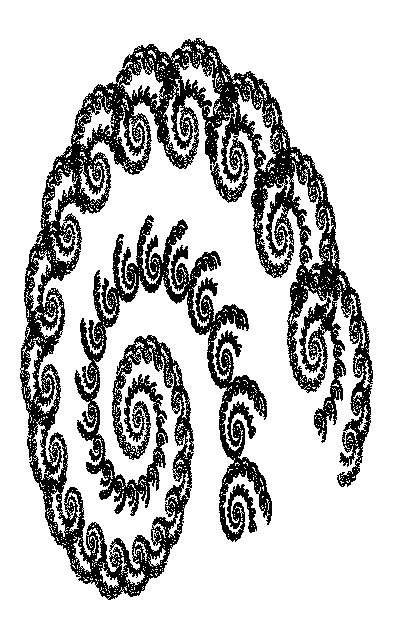
\includegraphics[width=0.42\textwidth]{fiddlehead}\hspace{1em}
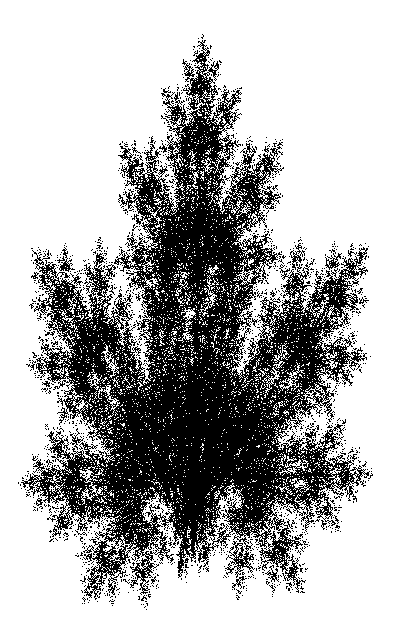
\includegraphics[width=0.42\textwidth]{maple}
\caption{Left: \texttt{fiddlehead}, a spiral of spirals from three maps
(Section~\ref{sec:spirals}). Right: \texttt{maple}, a classical four-map
leaf. Chaos game, $2\times 10^5$ points each.}
\label{fig:spirals}
\end{figure}

\subsection{Radial replication: umbels}
\label{sec:umbels}

The flower of the wild carrot (\emph{Daucus carota}, Queen Anne's lace) is
an \emph{umbel}: stalks radiate from one point to a domed rim, each stalk
ending in a smaller umbel, and so on for two or three botanical levels; the
attractor continues the recursion forever. The construction places $k$
shrunken, slightly rotated copies of the whole plant along the rim of a
dome, plus one stem map:
\begin{center}
\begin{tabular}{lllll}
\toprule
map & ratio $s$ & angle $\theta$ & translation & $p_i$ \\
\midrule
rim, far left  & $0.30$ & $-28^\circ$ & $(-0.70, 0.38)$ & $0.18$ \\
rim, left      & $0.36$ & $-14^\circ$ & $(-0.43, 0.50)$ & $0.18$ \\
rim, top       & $0.38$ & $0^\circ$   & $(0, 0.55)$     & $0.18$ \\
rim, right     & $0.36$ & $+14^\circ$ & $(0.43, 0.50)$  & $0.18$ \\
rim, far right & $0.30$ & $+28^\circ$ & $(0.70, 0.38)$  & $0.18$ \\
stem           & \multicolumn{2}{l}{$[\,0.02;0;0;0;0.55;0\,]$} & $(0,0)$ & $0.10$ \\
\bottomrule
\end{tabular}
\end{center}
The rotations lean the outer copies outward, following the dome's normal
directions, and the decreasing ratios toward the edge flatten the silhouette
exactly as gravity does for the plant. Thirty-six numbers in total
(Figure~\ref{fig:nature}, right).

Two design decisions carry the image. The first is that the ratios decrease
away from the centre ($0.38$ at the top, $0.30$ at the rim) while the
rotations increase ($0^\circ$ to $\pm 28^\circ$): equal ratios and no rotation
would produce a flat row of identical tufts, which reads as a diagram rather
than a flower, since real umbels are domes whose peripheral rays are both
shorter and tilted. The second is the choice of an odd number of rim maps.
With five, one map sits on the axis of symmetry and the two flanking pairs
mirror it, so the attractor inherits a single reflection axis, the bilateral
symmetry of a plant standing in gravity. A symmetry map would have been the
cheaper way to obtain regularity here, and it is exactly the wrong tool:
Proposition~\ref{prop:symmetry} would force full $C_k$ invariance, turning
the umbel into a rosette with no distinguished vertical and no place to
attach a stem.

\begin{figure}[t]
\centering
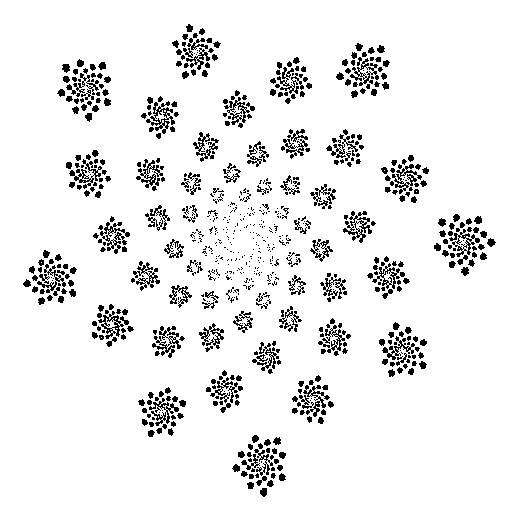
\includegraphics[width=0.42\textwidth]{sunflower}\hspace{1em}
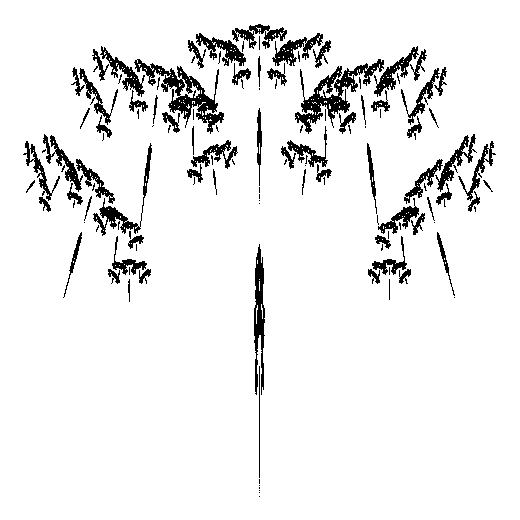
\includegraphics[width=0.42\textwidth]{lace}
\caption{Left: \texttt{sunflower}, golden-angle phyllotaxis from two maps
(Section~\ref{sec:phyllotaxis}), $5\times 10^5$ points. Right:
\texttt{lace}, an umbel of umbels from six maps (Section~\ref{sec:umbels}),
$3\times 10^5$ points.}
\label{fig:nature}
\end{figure}

\subsection{Golden-angle maps: phyllotaxis in two transforms}
\label{sec:phyllotaxis}

Sunflower heads, daisy capitula and romanesco spirals place successive
primordia at the \emph{golden angle} $\alpha = 360^\circ(1 - 1/\varphi) \approx
137.508^\circ$ from one another, where $\varphi$ is the golden ratio
\cite{vogel1979,prusinkiewicz1990}. Because $\varphi$ has continued fraction
$[1;1,1,\dots]$, it is the number worst approximated by rationals, so the
angles $k\alpha \bmod 360^\circ$ never lock onto spokes and fill the circle as
evenly as possible; this is the equidistribution that makes real seed heads
look uniformly packed.

The IFS rendition needs exactly two maps:
\begin{center}
\begin{tabular}{lllll}
\toprule
map & ratio $s$ & angle $\theta$ & translation & $p_i$ \\
\midrule
whorl & $0.97$ & $137.508^\circ$ & $(0,0)$ & $0.88$ \\
bud   & $0.13$ & $0^\circ$       & $(1,0)$ & $0.12$ \\
\bottomrule
\end{tabular}
\end{center}
The bud map plants a small copy of the whole attractor at the rim point
$(1,0)$; the whorl map sends bud $k$ to bud $k+1$, rotated by $\alpha$ and
pulled inward by $0.97$. The $k$-th bud therefore sits at angle $k\alpha$
and radius $0.97^{\,k}$, and since every bud is a copy of the whole
attractor, each is itself a rosette of rosettes (Figure~\ref{fig:nature},
left).

One honest caveat: real capitula follow Vogel's spiral $r = c\sqrt{k}$
\cite{vogel1979}, which keeps the areal density of organs constant, and the
computer graphics literature has since generalized it to arbitrary surfaces
of revolution \cite{ridley1986,prusinkiewicz2003}. An affine IFS can only
produce the geometric law $r = s^k$, since each application of the whorl map
multiplies the radius by a constant. Our attractor is thus a
\emph{logarithmic} phyllotaxis, denser toward the rim than a true sunflower;
the golden-angle equidistribution, which dominates the visual impression, is
nevertheless exact. It is worth noting that the golden angle itself is
empirical input in both models: it is reproduced, not explained
\cite{prusinkiewicz2003}.

\subsection{Symmetry maps: non-contracting members}
\label{sec:symmetry}

All previous maps were contractions. The last family is not: a \emph{pure
rotation at scale one},
\[
R \;=\; R(\beta), \qquad s_R = 1,
\]
included in the system with substantial probability. $R$ draws nothing new
by itself; in the chaos game it teleports the current point around the
attractor, replicating whatever the other maps produce into every rotated
position. It is a distribution-of-labour device: the contracting maps need
only describe \emph{one} sector of the figure, and $R$ propagates that
sector around the circle.

Hutchinson's theorem no longer applies, since $W$ is not a contraction on
$(\Hs, d_H)$. But the average contractivity condition \eqref{eq:average} is
easily satisfied: in the vegvísir system below, the rotation carries
probability $0.58$ and the remaining maps have ratios between $0.10$ and
$0.40$, giving $\sum_i p_i \ln s_i \approx -0.66 < 0$. Elton's theorem
\cite{elton1987} then guarantees a unique attracting invariant measure, and
the attractor, its support, still satisfies $A = \bigcup_i f_i(A)$.

The price is paid in rendering: since more than half of all chaos game steps
apply $R$, which revisits existing structure rather than refining it, the
attractor needs noticeably more iterations to fill in ($5\times 10^5$ where
the fern needs $2\times 10^5$). The probability $0.58$ was tuned
empirically: too low and the arms far from the generating sector stay
faint, too high and the contracting maps starve.

What a symmetry map can never do is break its own symmetry:

\begin{proposition}
\label{prop:symmetry}
Let $\{f_1,\dots,f_N\}$ with probabilities satisfying \eqref{eq:average}
contain a map $R$ that is a surjective isometry of $\R^2$ (e.g.\ a
rotation), and let $A = \operatorname{supp}\mu$ be the attractor. Then
$R(A) = A$.
\end{proposition}

\begin{proof}
From $A = \bigcup_i f_i(A) \supseteq R(A)$, the isometry $R$ maps the
compact set $A$ into itself. An isometry of a compact metric space into
itself is surjective: if some $x \in A$ had $d(x, R(A)) = \varepsilon > 0$,
the orbit $x_n = R^n(x)$ would satisfy $d(x_n, x_m) = d(x, R^{m-n}(x)) \ge
\varepsilon$ for all $m > n$, since $R^{m-n}(x) \in R(A)$; a sequence in a
compact set with no convergent subsequence is impossible. Hence
$R(A) = A$.
\end{proof}

With $\beta = 45^\circ$ the attractor is therefore invariant under the cyclic
group $C_8$: \emph{exactly} eightfold symmetric, whatever the other maps
do. This is both the power of the technique and, as the next section shows,
its limit.

\section{Case study: a designed symbol}
\label{sec:vegvisir}

The vegvísir is an Icelandic magical stave, a ``wayfinder'', known from
nineteenth-century manuscripts: eight arms radiate from a centre, and each
arm ends in a \emph{different} rune-like device. It is a natural challenge
for the vocabulary above: can an IFS draw it?

Strictly, no, and the obstruction is Proposition~\ref{prop:symmetry} read in
reverse. The economical way to draw eight arms is a $45^\circ$ symmetry map, but
then the attractor is exactly $C_8$-symmetric and all arms are congruent:
distinct terminal runes are ruled out. Renouncing the symmetry map does not
help at reasonable cost: each of the eight distinct rune motifs would need
its own group of maps, none of which may be an image of the whole (the
attractor equation $A = \bigcup f_i(A)$ forces every map's output to be a
copy of the entire symbol), so one is pushed toward IFS with condensation or
simply many dozens of coefficients, forfeiting the economy that makes the
exercise interesting. The deeper reason is aesthetic rather than technical:
the vegvísir was drawn by hand to \emph{mean} something, its asymmetry is
the content, and exact self-similarity has no room for it.

What an IFS can offer is a symmetric idealization
(Figure~\ref{fig:vegvisir}): an eight-armed rune star, every arm ending in
an infinitely recursive miniature of the whole. The system is six maps:

\begin{center}
\begin{tabular}{llll}
\toprule
map & coefficients $[\,a;b;c;d;e;f\,]$ & role & $p_i$ \\
\midrule
symmetry  & $[\,0.7071; -0.7071; 0; 0.7071; 0.7071; 0\,]$ & $R(45^\circ)$, $s=1$ & $0.58$ \\
shaft     & $[\,0.40; 0; 0.45; 0; 0.04; 0\,]$ & stem map, horizontal & $0.18$ \\
crossbar 1 & $[\,0; -0.11; 0.55; 0.11; 0; 0\,]$ & $0.11\,R(90^\circ)$ at $x{=}0.55$ & $0.08$ \\
crossbar 2 & $[\,0; -0.15; 0.82; 0.15; 0; 0\,]$ & $0.15\,R(90^\circ)$ at $x{=}0.82$ & $0.08$ \\
tip       & $[\,0.10; 0; 1.00; 0; 0.10; 0\,]$ & miniature at arm's end & $0.05$ \\
centre    & $[\,0.18; 0; 0; 0; 0.18; 0\,]$ & miniature at origin & $0.03$ \\
\bottomrule
\end{tabular}
\end{center}

The five contracting maps describe a single horizontal arm: a flat shaft
(Section~\ref{sec:stems}), two rotated crossbar copies whose own eightfold
structure decorates them with rune-like detail, a tip miniature, and a
centre filler. The symmetry map replicates the arm eight times. The result
is not a vegvísir; it is what the vegvísir would be if it were grown by a
rule instead of drawn by a hand, and the family resemblance is exactly the
part of the symbol that is rule-like.

\begin{figure}[t]
\centering
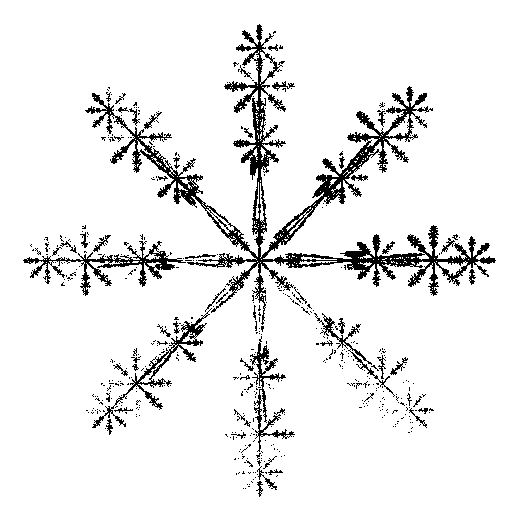
\includegraphics[width=0.40\textwidth]{vegvisir}
\caption{The \texttt{vegvisir} attractor: six maps, $C_8$-symmetric by
Proposition~\ref{prop:symmetry}. Chaos game, $5\times 10^5$ points.}
\label{fig:vegvisir}
\end{figure}

\section{Why nature cooperates}
\label{sec:nature}

Half of the attractors above depict plants, and they are by a wide margin
the most convincing ones. The library's history repeats the observation:
of its sixteen attractors, the memorable ones are the fern, the maple
leaf, the tree, the fiddlehead, the sunflower, the wild carrot; the
geometric and symbolic ones read as diagrams. The explanation is not that
plants are pretty, but that the encoding fits.

A plant does not execute a blueprint of its final shape. It grows by
repeating local rules: sprout, shrink, turn, branch. Its adult form is the
accumulation of one rule applied at every scale, which is precisely the
fixed point equation $A = \bigcup_i f_i(A)$. Developmental biology
formalizes the same observation as L-systems, parallel rewriting systems in
which each module of the organism is advanced by rules depending only on its
own state and its neighbours \cite{prusinkiewicz1990}; in the vocabulary of
\cite{prusinkiewicz2003}, a growing plant is a \emph{structured dynamical
system} whose transition function is local. Locality plus repetition is
self-similarity. The fern is not \emph{like} a fractal; within the
resolution at which physiology cuts off the recursion, it \emph{is} the
attractor of a handful of affine maps, which is why Barnsley could capture
it in twenty-four coefficients \cite{barnsleydemko1985}. The romanesco that
illustrated self-similarity in the author's 2008 report
\cite{bonhomme2008paysagesfractals} makes the same point in three dimensions, and its
golden-angle spirals are the ones distilled into the two-map system of
Section~\ref{sec:phyllotaxis}.

The comparison also marks the boundary of what an IFS can say. An L-system
models development \emph{in time}, and its later refinements add exactly the
ingredients an IFS lacks: context sensitivity, positional information along
an axis, competition for light and space, and biomechanics
\cite{prusinkiewicz2003}. An IFS keeps only the limit of that process, and
only when the process is context-free and strictly self-similar. Our
\texttt{lace} is an idealized umbel whose every ray is a copy of the whole,
whereas a real \emph{Daucus carota} has rays that shorten toward the rim
under positional control; the attractor buys its thirty-six coefficients by
discarding that regulation. The right reading is not that plants are IFS,
but that the deterministic, context-free core of plant development is
exactly the part an IFS can capture, and that this core already accounts for
most of what makes a fern look like a fern.

Designed artifacts sit at the other pole. A symbol like the vegvísir is
drawn once, at one scale, to carry meaning; nothing in its production
iterates, and Section~\ref{sec:vegvisir} showed how the mathematics
enforces the mismatch. Between the two poles lie nature's
\emph{statistically} self-similar forms: coastlines, clouds, mountain
relief. These grow by iteration too, but by noisy iteration, and their
proper tools are the random constructions (midpoint displacement, fractional
Brownian surfaces) surveyed in \cite{mandelbrot1982,bonhomme2008paysagesfractals}; a
deterministic IFS renders them as too regular, just as it renders the
vegvísir as too symmetric. The rule of thumb the vocabulary suggests is
simple: exact self-similarity for what grows by a deterministic rule,
randomness for what grows by a noisy one, and resignation for what does not
grow at all.

\section{Implementation notes}
\label{sec:implementation}

Everything above is implemented in \texttt{ifs-fractals}
\cite{ifsfractals2026}, an OCaml library and command-line tool (about two
hundred lines in total, chaos game included) released under the GPL and
distributed through opam:

\begin{lstlisting}
$ opam install ifs-fractals
$ ifs-fractals lace
\end{lstlisting}

\noindent
The design loop deserves a methodological remark, since it is what makes the
vocabulary usable in practice. Coefficients were never written blind: each
candidate system was first simulated (a Python port of the chaos game, a few
dozen lines), rendered to an image, inspected, and iterated upon; the
simulation also computed the attractor's bounding box, which becomes the
viewport stored with the system. The loop from a parametric family of
Section~\ref{sec:vocabulary} to shipped coefficients took minutes per
attractor. Readers wishing to extend the collection will find that the
vocabulary plus this simulate-inspect loop makes the inverse problem, if not
solved, at least workmanlike.

\subsection*{Use of a language model}

The six new attractors were designed in 2026 in an interactive session with
Claude Fable~5, a large language model by Anthropic, and it would be
misleading to describe the division of labour vaguely. The author set the
goals and constraints, ran and inspected the renderings, decided which
candidates to keep, and checked the statements made here; the model proposed
the botanical subjects, derived and tuned the coefficient sets inside the
simulate-inspect loop above, and drafted the exposition, including the proof
of Proposition~\ref{prop:symmetry}. Responsibility for the correctness of the
mathematics and for the final content rests with the author; the model is a
tool, not an author.

Two of its behaviours are worth recording for readers considering the same
workflow. Asked for the vegvísir, it identified the obstruction of
Section~\ref{sec:vegvisir} \emph{before} attempting a construction, rather
than returning a plausible but wrong system; and asked whether
\texttt{fiddlehead} was original, it traced the architecture back to the
\texttt{galaxy} attractor already present in the library, which is the
provenance reported in Section~\ref{sec:spirals}. A narrative account of the
sessions is given in \cite{bonhomme2026blog}.

\section{Conclusion}

Affine IFS design is usually presented as a gallery of received coefficient
tables. Naming the construction techniques (stem maps, spiral generators,
radial replication, golden-angle maps, symmetry maps) turns the gallery into
a grammar: the six attractors added to a sixteen-year-old library in 2026 were
all obtained by composing these families and tuning by inspection, in minutes
each. The
grammar also knows its own limits, and states one of them precisely:
Proposition~\ref{prop:symmetry} says that the cheap way to eightfold
symmetry forecloses any asymmetric content, which is why grown forms fit in
a few dozen coefficients while a hand-drawn symbol never will. The gap
between a fern and a vegvísir is not twenty-four coefficients; it is the
difference between form produced by iteration and form produced by
intention.

\bibliographystyle{alpha}
\bibliography{refs}

\end{document}
